\documentclass[10pt]{beamer}

\usetheme{metropolis}
\usepackage{appendixnumberbeamer}

\usepackage{booktabs}
\usepackage[scale=2]{ccicons}
\usepackage{pgfplots}
\usepgfplotslibrary{dateplot}

\usepackage{xspace}
\newcommand{\themename}{\textbf{\textsc{metropolis}}\xspace}

\usepackage{stmaryrd}
\usepackage{amsmath}


\usepackage{tikz}
\usepackage{siunitx}
\usetikzlibrary{calc,decorations.pathmorphing,patterns}

%%%%%%%%%%%%%%%%%%%%%%%%%%%%%%%%%%%%%%%%%%%%%%%%%%%%%%%%%%%%%%%%%%%%%%%%%
%%%% The following is for fancy box %%%%%%%%%%%%%%
\usepackage[framemethod=TikZ]{mdframed}
%%%%%%%%%%%%% Theorem %%%%%%%%%%%%
\newenvironment{thm}[2][]{%
\ifstrempty{#1}%
{\mdfsetup{%
frametitle={%
\tikz[baseline=(current bounding box.east),outer sep=0pt]
\node[anchor=east,rectangle,fill=red!20]
{\strut Theorem};}}
}%
{\mdfsetup{%
frametitle={%
\tikz[baseline=(current bounding box.east),outer sep=0pt]
\node[anchor=east,rectangle,fill=red!20]
{\strut Theorem #1};}}%
}%
\mdfsetup{innertopmargin=1pt,linecolor=red!20,%
linewidth=2pt,topline=true,%
frametitleaboveskip=\dimexpr-\ht\strutbox\relax
}
\begin{mdframed}[]\relax%
\label{#2}}{\end{mdframed}}
%%%%%%%%%%%%%%Lemma%%%%%%%%%%%%%%%%%%%%%%%%%%%%%%%%%%%%%%%%%%%%%%%%%%%%%%
\newcounter{lem}[section] \setcounter{lem}{0}
\renewcommand{\thelem}{\arabic{section}.\arabic{lem}}
\newenvironment{lem}[2][]{%
\refstepcounter{lem}%
\ifstrempty{#1}%
{\mdfsetup{%
frametitle={%
\tikz[baseline=(current bounding box.east),outer sep=0pt]
\node[anchor=east,rectangle,fill=green!20]
{\strut Lemma~\thelem};}}
}%
{\mdfsetup{%
frametitle={%
\tikz[baseline=(current bounding box.east),outer sep=0pt]
\node[anchor=east,rectangle,fill=green!20]
{\strut Lemma~\thelem:~#1};}}%
}%
\mdfsetup{innertopmargin=1pt,linecolor=green!20,%
linewidth=2pt,topline=true,%
frametitleaboveskip=\dimexpr-\ht\strutbox\relax
}
\begin{mdframed}[]\relax%
\label{#2}}{\end{mdframed}}
%%%%%%%%%%%%%%%%%%%%%%%%%%%%%%%%%%%%%%%%%%%%%%%%%%%%%%%%%%%%%%%%%%%%%%%
%Proof
\newenvironment{prove}[2][]{%
\ifstrempty{#1}%
{\mdfsetup{%
frametitle={%
\tikz[baseline=(current bounding box.east),outer sep=0pt]
\node[anchor=east,rectangle,fill=red!20]
{\strut Proof};}}
}%
{\mdfsetup{%
frametitle={%
\tikz[baseline=(current bounding box.east),outer sep=0pt]
\node[anchor=east,rectangle,fill=red!20]
{\strut Proof:~#1};}}%
}%
\mdfsetup{innertopmargin=1pt,linecolor=red!20,%
linewidth=2pt,topline=true,%
frametitleaboveskip=\dimexpr-\ht\strutbox\relax
}
\begin{mdframed}[]\relax%
\label{#2}}{\end{mdframed}}
%%%%%%%%%%%%%%%%%%%%%%%%%%%%%%%%%%%%%%%%%%%%%%%%%%%%%%%%%%%%%%%%%%%%%%%
%Defintion
\newcounter{drf}[section]\setcounter{drf}{0}
\renewcommand{\thedrf}{}
\newenvironment{drf}[2][]{%
\refstepcounter{drf}%
\ifstrempty{#1}%
{\mdfsetup{%
frametitle={%
\tikz[baseline=(current bounding box.east),outer sep=0pt]
\node[anchor=east,rectangle,fill=orange!20]
{\strut Definition~\thedrf};}}
}%
{\mdfsetup{%
frametitle={%
\tikz[baseline=(current bounding box.east),outer sep=0pt]
\node[anchor=east,rectangle,fill=orange!20]
{\strut Definition~\thedrf:~#1};}}%
}%
\mdfsetup{innertopmargin=1pt,linecolor=orange!20,%
linewidth=2pt,topline=true,%
frametitleaboveskip=\dimexpr-\ht\strutbox\relax
}
\begin{mdframed}[]\relax%
\label{#2}}{\end{mdframed}}
%%%%%%%%%%%%%%%%%%%%%%%%%%%%%%%%%%%%%%%%%%%%%%%%%%%%%%%%%%%%%%%%%%%%%%%%%%%
% end of self defined label
%%%%%%%%%%%%%%%%%%%%%%%%%%%%%%%%%%%%%%%%%%%%%%%%%%%%%%%%%%%%%%%%%%%%%%%%%%%


%%%%%%%%%%%%%% For double curly bracket%%%%%%%%%%%%%%%%
\usepackage{xparse}

\NewDocumentCommand{\dgal}{sO{}m}{%
  \IfBooleanTF{#1}
    {\dgalext{#3}}
    {\dgalx[#2]{#3}}%
}

\NewDocumentCommand{\dgalext}{m}{%
  \sbox0{%
    \mathsurround=0pt % just for safety
    $\left\{\vphantom{#1}\right.\kern-\nulldelimiterspace$%
  }%
  \sbox2{\{}%
  \ifdim\ht0=\ht2
    \{\kern-.45\wd2 \{#1\}\kern-.45\wd2 \}%
  \else
    \left\{\kern-.5\wd0\left\{#1\right\}\kern-.5\wd0\right\}%
  \fi
}

\NewDocumentCommand{\dgalx}{om}{%
  \sbox0{\mathsurround=0pt$#1\{$}%
  \sbox2{\{}%
  \ifdim\ht0=\ht2
    \{\kern-.45\wd2 \{#2\}\kern-.45\wd2 \}%
  \else
    \mathopen{#1\{\kern-.5\wd0 #1\{}
    #2
    \mathclose{#1\}\kern-.5\wd0 #1\}}
  \fi
}
%%%%%%%%%%%%%%%%



%%%%%%%%%%%%%%%%%%%%%%%%%%%%%%%%%%%%%

\usepackage{animate}

\graphicspath{{./fig/}}


%%%%%%%%%%%%%% define color %%%%%%%%%%%%%%%%%%
\definecolor{DarkFern}{HTML}{407428}
\definecolor{DarkCharcoal}{HTML}{4D4944}
\colorlet{Fern}{DarkFern!85!white}
\colorlet{Charcoal}{DarkCharcoal!85!white}
\colorlet{LightCharcoal}{Charcoal!50!white}
\colorlet{AlertColor}{orange!80!black}
\colorlet{DarkRed}{red!70!black}
\colorlet{DarkBlue}{blue!70!black}
\colorlet{DarkGreen}{green!70!black}

\newcommand{\I}{\mathrm{i}}




%%%%%%%%%%%%%%%%%%%%%%%%%%%%%%%%%%%%%%
%\newcommand{\G}{\alert{G}}  % change color of main author



%%%%%%%%%%%%% Title Page %%%%%%%%%%%%%%%%%%%

\title{MAST90026 Computational Differential\\Equations: Week 1}
%\subtitle{A modern beamer theme}
\date{Semester 1 2024}
\author{Jesse Collis\\Modified from Hailong Guo (2022)}
\institute{The University of Melbourne}
\titlegraphic{\vspace{6cm}\flushright\includegraphics[height=2cm]{logo.png}}


\begin{document}

\maketitle





%-=-=-=-=-=-=-=-=-=-=-=-=-=-=-=-=-=-=-=-=-=-=-=-=
%	FRAME:
%-=-=-=-=-=-=-=-=-=-=-=-=-=-=-=-=-=-=-=-=-=-=-=-=
\begin{frame}{Goal of the subject}

  Cover numerical techniques for solving 
  \begin{itemize}
  	\item Boundary value problems (BVPs) for ODEs
  	\item Simple PDEs 
  	\begin{itemize}
  	\item 2D Elliptic PDES
  	\item 1+1 (1 space dimension, 1 time dimension) parabolic, hyperbolic
  	\end{itemize}
  	\item Sparse solvers for linear systems 
  \end{itemize}  
    
	
\end{frame}



%-=-=-=-=-=-=-=-=-=-=-=-=-=-=-=-=-=-=-=-=-=-=-=-=
%	FRAME:
%-=-=-=-=-=-=-=-=-=-=-=-=-=-=-=-=-=-=-=-=-=-=-=-=
\begin{frame}{Model equation}


\begin{overprint}
	\onslide<1->{
\only<1>{ 
  Convection-diffusion equation:
  \begin{equation*}
  	u_t+\vec{v}\cdot\nabla u=\nabla\cdot(\operatorname{D}\nabla u)+f.
  \end{equation*}
    

 
$
\nabla = (\frac{\partial}{\partial x}, \frac{\partial}{\partial y})
 $
 
\vspace{0.05in}
$ \vec{v}, D>0, f$ given functions of $(x, y)$

Scalar, linear parabolic equation
}
\only<2>{

 Limiting cases $\vec{v}=\vec{0}$: Heat equation
  \begin{equation*}
  	u_t =\nabla\cdot(\operatorname{D}\nabla u)+f.
  \end{equation*}
     

1D heat equation:
  \begin{equation*}
  	u_t = Du_{xx}+f.
  \end{equation*}
}


\only<3>{

 Limiting cases $D=0$: Advection/transport/1-way wave equation
  \begin{equation*}
  	u_t+\vec{v}\cdot\nabla u=f.
  \end{equation*}
 
 1D hyperbolic equation:
  \begin{equation*}
  	u_t + vu_{x}+f.
  \end{equation*}  

}



\only<4>{

 Limiting cases $u_t=0$ (steady state): elliptic equation
  \begin{equation*}
  	\vec{v}\cdot\nabla u= \nabla\cdot(\operatorname{D}\nabla u) + f.
  \end{equation*}
    
  Further $\vec{v}=\vec{0} \rightarrow$ Poisson equation
  
   \begin{equation*}
  	-\nabla\cdot(\operatorname{D}\nabla u) = f.
  \end{equation*}
  
  
  1D elliptic equation
  \begin{equation*}
  	vu_x= \operatorname{D}u_{xx} + f.
  \end{equation*}
}



}
\end{overprint}



	
\end{frame}








%-=-=-=-=-=-=-=-=-=-=-=-=-=-=-=-=-=-=-=-=-=-=-=-=
%	FRAME:
%-=-=-=-=-=-=-=-=-=-=-=-=-=-=-=-=-=-=-=-=-=-=-=-=
\begin{frame}{Issues}

   How do we iterate in time (for IVPs)?
   
   \vspace{0.3em}
   
   How do we represent the solution in space (for BVPs/PDEs)?
   
      \vspace{0.3em}

   
   How do we handle higher dimensionality?
   
   
      \vspace{0.3em}

   How do we handle non-linearities?
    
   	
\end{frame}



%-=-=-=-=-=-=-=-=-=-=-=-=-=-=-=-=-=-=-=-=-=-=-=-=
%	FRAME:
%-=-=-=-=-=-=-=-=-=-=-=-=-=-=-=-=-=-=-=-=-=-=-=-=
\begin{frame}{2nd order BVPs}


Linear BVP
\begin{equation*}
	-u'' + p(x)u' + q(x)u = r(x), x\in[a, b]
\end{equation*}
 with  linear separated  boundary condition (Robin boundary condition)
\begin{align*}
	&A_{11}u(a) + A_{12}u'(a) = \beta_1, \\
	&A_{21}u(b) + A_{22}u'(b) = \beta_2.
\end{align*} 
    
   	
\end{frame}



%-=-=-=-=-=-=-=-=-=-=-=-=-=-=-=-=-=-=-=-=-=-=-=-=
%	FRAME:
%-=-=-=-=-=-=-=-=-=-=-=-=-=-=-=-=-=-=-=-=-=-=-=-=
\begin{frame}{More general 2nd order BVPs}


General form
\begin{equation*}
	u'' = f(x, u, u'),
\end{equation*}
 with  separated  boundary condition at $x=a$ and $x=b$
 \begin{align*}
	&g_1(u(a),u'(a)) = B_1, \\
	&g_2(u(b),u'(b)) = \beta_2.
\end{align*} 
    
 
 
 Note linear BVPs could have $0$, $1$, or $\infty$ many solutions.    
    
    
   	
\end{frame}



%-=-=-=-=-=-=-=-=-=-=-=-=-=-=-=-=-=-=-=-=-=-=-=-=
%	FRAME:
%-=-=-=-=-=-=-=-=-=-=-=-=-=-=-=-=-=-=-=-=-=-=-=-=
\begin{frame}{Existing methods for boundary value problems}

    
    \begin{center}
  \includegraphics[width=1.03\textwidth]{BVPs.pdf}
     \end{center}
    

   % \begin{tikzpicture}[remember picture, overlay]
    %    \draw[ultra thick,color=red] (0,0) -- (11,7) (11,0) -- (0,7);
    %\end{tikzpicture}
	
\end{frame}


%-=-=-=-=-=-=-=-=-=-=-=-=-=-=-=-=-=-=-=-=-=-=-=-=
%	FRAME:
%-=-=-=-=-=-=-=-=-=-=-=-=-=-=-=-=-=-=-=-=-=-=-=-=
\begin{frame}{General principle}

    
   Consider 
   \begin{equation*}
   	Lu = r(x)
   \end{equation*}
    where $L$ is a linear operator involving derivatives. 
    
    
    \vspace{0.8em}
    
The main difference between finite difference methods(FDMs) and weighted residual methods (WRMs):
\begin{enumerate}
	\item For FDM, approximate the differential operator $L$.
	\item For WRMs, approximate the solution $u$. 
\end{enumerate}    




  
\end{frame}



%-=-=-=-=-=-=-=-=-=-=-=-=-=-=-=-=-=-=-=-=-=-=-=-=
%	FRAME:
%-=-=-=-=-=-=-=-=-=-=-=-=-=-=-=-=-=-=-=-=-=-=-=-=
\begin{frame}{Finite difference formulae}
Idea: Approximate $u'$ and $u''$. 


\vspace{0.5em}
Only approximate derivatives at selected points: $h = \frac{b-a}{N+1}$ and $ x_j = a + jh$
\begin{center}
	    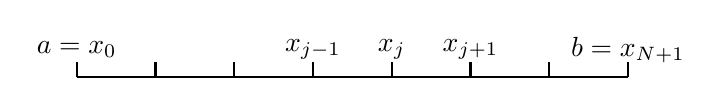
\begin{tikzpicture}
  \draw[color=black, thick] (0,0) -- (1, 0) -- (2, 0) -- (3, 0) -- (4, 0) -- (5, 0) -- (6, 0) -- (7, 0);
  \foreach \x in {0,...,7}
  {
  \draw[color=black, thick] (\x, 0) -- (\x, 0.2);
  }
  \node at (0, 0.35) {$a = x_0$};
    \node at (7, 0.35) {$b = x_{N+1}$};
     \node at (3, 0.35) {$ x_{j-1}$};
      \node at (4, 0.35) {$ x_{j}$};
       \node at (5, 0.35) {$x_{j+1}$};

\end{tikzpicture}

\end{center}


\vspace{0.4em}
Can also use nonuniform meshes $\{x_j\}$ with $h_j = x_{j+1}-x_j$.\\

  
\end{frame}




%-=-=-=-=-=-=-=-=-=-=-=-=-=-=-=-=-=-=-=-=-=-=-=-=
%	FRAME:
%-=-=-=-=-=-=-=-=-=-=-=-=-=-=-=-=-=-=-=-=-=-=-=-=
\begin{frame}{Some examples}


For $u'$:
\begin{itemize}
	\item Forward difference: $u'(x) = \frac{u(x+h)-u(x)}{h}+\text{error}$.
	\item Backward difference: $u'(x) = \frac{u(x)-u(x-h)}{h}+\text{error}$.
	\item Central difference: $u'(x) = \frac{u(x+h)-u(x-h)}{2h}+\text{error}$.
\end{itemize}

\vspace{0.5em}
For $u''$:
\begin{itemize}
	\item Central difference: $u''(x) = \frac{u(x+h)-2u(x)+u(x-h)}{h^2}+\text{error}$.
\end{itemize}

\end{frame}


%-=-=-=-=-=-=-=-=-=-=-=-=-=-=-=-=-=-=-=-=-=-=-=-=
%	FRAME:
%-=-=-=-=-=-=-=-=-=-=-=-=-=-=-=-=-=-=-=-=-=-=-=-=
\begin{frame}{General finite difference scheme}



In general, approximate $u^{(k)}$ as
\begin{equation*}
u^{(k)}(x) =  \sum_{i=1}^n c_i u(x+h_i) +\text{error}.
\end{equation*}


\vspace{0.2em}

Derivation:
\begin{itemize}
	\item The method of underdetermined coefficient (Taylor series expansion)
	\item Interpolation and then differentiation
\end{itemize}


\vspace{0.2em}
Error for interpolating using n points is $\mathcal{O}(h^n)$. The worst-case error for approximating $u^{(k)}$ is $\mathcal{O}(h^{n-k})$. 



  
\end{frame}




%-=-=-=-=-=-=-=-=-=-=-=-=-=-=-=-=-=-=-=-=-=-=-=-=
%	FRAME:
%-=-=-=-=-=-=-=-=-=-=-=-=-=-=-=-=-=-=-=-=-=-=-=-=
\begin{frame}{Discretizaiton error}



Central finite difference error:

\begin{align*}
&\frac{u(x+h)-u(x-h)}{2h}\\
=&\frac{1}{2h}\left(u(x)+hu'(x)+\frac{1}{2}h^2 u''(x)+O(h^3)\right)-\\
&\frac{1}{2h}\left(u(x)-hu'(x)+\frac{1}{2}h^2 u''(x)+O(h^3)\right)\\
=&\frac{2hu'(x)+O(h^3)}{2h}\\
=&u'(x)+O(h^2),
\end{align*}



Similarly, the error for FD, BD, CD for $u''$. 

  
\end{frame}


%-=-=-=-=-=-=-=-=-=-=-=-=-=-=-=-=-=-=-=-=-=-=-=-=
%	FRAME:
%-=-=-=-=-=-=-=-=-=-=-=-=-=-=-=-=-=-=-=-=-=-=-=-=
\begin{frame}{FDM for BVPs}



Consider 
\begin{align*}
&u''(x)+p(x)u'(x)+q(x)u(x)=r(x),\\
&u(a)=\alpha, u(b)=\beta.
\end{align*}


\vspace{0.2em}


Consider  $h = \frac{b-a}{N+1}$ and $ x_j = a + jh$:
\begin{center}
	    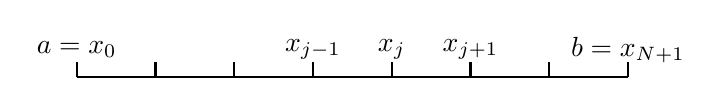
\begin{tikzpicture}
  \draw[color=black, thick] (0,0) -- (1, 0) -- (2, 0) -- (3, 0) -- (4, 0) -- (5, 0) -- (6, 0) -- (7, 0);
  \foreach \x in {0,...,7}
  {
  \draw[color=black, thick] (\x, 0) -- (\x, 0.2);
  }
  \node at (0, 0.35) {$a = x_0$};
    \node at (7, 0.35) {$b = x_{N+1}$};
     \node at (3, 0.35) {$ x_{j-1}$};
      \node at (4, 0.35) {$ x_{j}$};
       \node at (5, 0.35) {$x_{j+1}$};

\end{tikzpicture}

\end{center}

\vspace{0.2em}


\alert{Idea}: Use central difference approximation for $u'$ and $u''$ at $x_j$:
\begin{equation*}
\frac{u_{j+1}-2u_j+u_{j-1}}{h^2}+p(x_j)\frac{u_{j+1}-u_{j-1}}{2h}+q(x_j)u_j=r(x_j).
\end{equation*}





  
\end{frame}



%-=-=-=-=-=-=-=-=-=-=-=-=-=-=-=-=-=-=-=-=-=-=-=-=
%	FRAME:
%-=-=-=-=-=-=-=-=-=-=-=-=-=-=-=-=-=-=-=-=-=-=-=-=
\begin{frame}{Linear system for FDM}

Let $p(x_j)=p_j$, $q(x_j)=q_j$ and $r(x_j)=r_j$.

\begin{align*}
u_0=\alpha,\\
\frac{u_0-2u_1+u_2}{h^2}+p_1\frac{u_2-u_0}{2h}+q_1 u_1=r_1,\\
\frac{u_1-2u_2+u_3}{h^2}+p_2\frac{u_3-u_1}{2h}+q_2 u_2=r_2,\\
\vdots\\
\frac{u_{N-1}-2u_N+u_{N+1}}{h^2}+p_N\frac{u_{N+1}-u_{N-1}}{2h}+q_N u_N=r_N,\\
u_{N+1}=\beta.
\end{align*}


\end{frame}



%-=-=-=-=-=-=-=-=-=-=-=-=-=-=-=-=-=-=-=-=-=-=-=-=
%	FRAME:
%-=-=-=-=-=-=-=-=-=-=-=-=-=-=-=-=-=-=-=-=-=-=-=-=
\begin{frame}{Simplification of Linear system for FDM}

Change the second and second last equation to:
\begin{align*}
\frac{-2u_1+u_2}{h^2}+p_1\frac{u_2}{2h}+q_1 u_1=r_1-\frac{\alpha}{h^2}+p_1\frac{\alpha}{2h},\\
\frac{u_{N-1}-2u_N}{h^2}+p_N\frac{-u_{N-1}}{2h}+q_N u_N=r_N - \frac{\beta}{h^2}-p_N\frac{\beta}{2h}.
\end{align*}


\end{frame}



%-=-=-=-=-=-=-=-=-=-=-=-=-=-=-=-=-=-=-=-=-=-=-=-=
%	FRAME:
%-=-=-=-=-=-=-=-=-=-=-=-=-=-=-=-=-=-=-=-=-=-=-=-=
\begin{frame}{Matrix form}

\begin{align*}
\frac{1}{h^2}
&\begin{pmatrix}
-2+h^2q_1 &1+h\frac{p_1}{2}&0 &0\\
1-h\frac{p_2}{2} &\ddots &\ddots &0\\
0 &\ddots &\ddots &1+h\frac{p_{N-1}}{2}\\
0& 0& 1-h\frac{p_N}{2} &-2 +h^2 q_N
\end{pmatrix}
\begin{pmatrix}
u_1\\
u_2\\
\vdots\\
u_N
\end{pmatrix}
\\
=&
\begin{pmatrix}
r_1-\frac{\alpha}{h^2}+p_1\frac{\alpha}{2h}\\
r_2\\
\vdots\\
r_N-\frac{\beta}{h^2}-p_N\frac{\beta}{2h}
\end{pmatrix}
\end{align*}


\end{frame}



%-=-=-=-=-=-=-=-=-=-=-=-=-=-=-=-=-=-=-=-=-=-=-=-=
%	FRAME:
%-=-=-=-=-=-=-=-=-=-=-=-=-=-=-=-=-=-=-=-=-=-=-=-=
\begin{frame}{Questions to ask  }



1. Does this have a solution?
 \vspace{0.2em}

 
2.  How hard is it to solve?

\vspace{0.2em}

 
3. How well does $\bf{u}$ approximate $u(x)$ for a given $h$?
 
 
 \vspace{0.2em}

4. Does $u_j \to u(x_j)$ as $h \to 0$?

\end{frame}






%-=-=-=-=-=-=-=-=-=-=-=-=-=-=-=-=-=-=-=-=-=-=-=-=
%	FRAME:
%-=-=-=-=-=-=-=-=-=-=-=-=-=-=-=-=-=-=-=-=-=-=-=-=
\begin{frame}{Measure the error  }




The grid function (i.e. it is only defined on the grid/mesh) norms:
\begin{align*}
&\| \Sigma \|_1= h \sum|\Sigma_i|,\\
&\| \Sigma \|_2 = \left(h \sum|\Sigma_i|^2 \right)^{\frac{1}{2}},\\
&\| \Sigma \|_\infty = \operatorname{max}|\Sigma_i|. 
\end{align*}

% \vspace{0.2em}

Define the global error:
\begin{equation*}
 \| E \| =  \| \mathbf{u} - \hat{\mathbf{u}} \|.
\end{equation*}




\end{frame}







%-=-=-=-=-=-=-=-=-=-=-=-=-=-=-=-=-=-=-=-=-=-=-=-=
%	FRAME:
%-=-=-=-=-=-=-=-=-=-=-=-=-=-=-=-=-=-=-=-=-=-=-=-=
\begin{frame}{Some terminologies   }




\begin{drf} [Convergence]
	 A A method with global error $\| E\|=O(h^p)$ as $h \to 0$ is convergent of order $p$.
\end{drf}



\begin{drf} [Local Truncation Error (LTE)]
	 A The local truncation error $\tau_j$ is the residual at grid point $x_j$ when the true solution is put into the finite difference formula.
\end{drf}



\begin{drf} [Consistency]
	 A A method is consistent of order $p$ if \mbox{$\|\tau\| = O(h^p)$} as $h \to 0$.
\end{drf}

\end{frame}




%-=-=-=-=-=-=-=-=-=-=-=-=-=-=-=-=-=-=-=-=-=-=-=-=
%	FRAME:
%-=-=-=-=-=-=-=-=-=-=-=-=-=-=-=-=-=-=-=-=-=-=-=-=
\begin{frame}{LTE for our system  }

\begin{equation*}
	\begin{split}	
	\tau_j = &\frac{1}{h^2}(u(x_{j+1})-2u(x_j)+u(x_{j-1}))+p(x_j)\frac{u(x_{j+1})-
	u(x_{j-1})}{2h}+\\
	&q(x_j)u(x_j)-r(x_j)\\
	=&u''(x_j)+p(x_j)u'(x_j)+q(x_j)u(x_j)-r(x_j)+ C h^2u^{(3)}+O(h^4)\\
=&C h^2u^{(3)}(\xi)+O(h^4),
	\end{split}
\end{equation*}



\end{frame}





%-=-=-=-=-=-=-=-=-=-=-=-=-=-=-=-=-=-=-=-=-=-=-=-=
%	FRAME:
%-=-=-=-=-=-=-=-=-=-=-=-=-=-=-=-=-=-=-=-=-=-=-=-=
\begin{frame}{Error equation }

 Original scheme
 \[  A  \mathbf{u} = \mathbf{b}.  \]

 \vspace{0.2em}
 

Consistency 
\[ A  \hat{\mathbf{u}} = \mathbf{b} + \tau. \]


 \vspace{0.2em}


The global error $\mathbf{E} =  \mathbf{u} - \hat{\mathbf{u}} $ satisfies 
\[
A( \mathbf{u} - \hat{\mathbf{u}}) = -\tau
\]



\end{frame}


%-=-=-=-=-=-=-=-=-=-=-=-=-=-=-=-=-=-=-=-=-=-=-=-=
%	FRAME:
%-=-=-=-=-=-=-=-=-=-=-=-=-=-=-=-=-=-=-=-=-=-=-=-=
\begin{frame}{Convergence }


Error equation

\[
\mathbf{E} =  -A^{-1}\tau.
\]

Taking norms
\begin{align*}
	\|\mathbf{E}\| =  &\| -A^{-1}\tau\|\\
	               \le & \|A^{-1}\|\|\tau\|\\
	               \le & \|A^{-1}\|Ch^2. 
\end{align*}


\end{frame}



%-=-=-=-=-=-=-=-=-=-=-=-=-=-=-=-=-=-=-=-=-=-=-=-=
%	FRAME:
%-=-=-=-=-=-=-=-=-=-=-=-=-=-=-=-=-=-=-=-=-=-=-=-=
\begin{frame}{Summary }


\begin{center}
	Consistency $+$ Stability $\Rightarrow$ Convergence 
\end{center}



%\begin{equation*}
%\begin{array}[ccccc]
%	Convergence & + & Stability & \Rightarrow & Convergence
%\end{array}	
%\end{equation*}
%


\end{frame}




%-=-=-=-=-=-=-=-=-=-=-=-=-=-=-=-=-=-=-=-=-=-=-=-=
%	FRAME:
%-=-=-=-=-=-=-=-=-=-=-=-=-=-=-=-=-=-=-=-=-=-=-=-=
\begin{frame}{Other type boundary condition }
Taking $u'(x_0)=\alpha$ as an exmaple.

   
    \begin{center}
  \includegraphics[width=1.03\textwidth]{handlebc.pdf}
     \end{center}


\end{frame}




%-=-=-=-=-=-=-=-=-=-=-=-=-=-=-=-=-=-=-=-=-=-=-=-=
%	FRAME:
%-=-=-=-=-=-=-=-=-=-=-=-=-=-=-=-=-=-=-=-=-=-=-=-=
\begin{frame}{Ghost point method}

\begin{center}
	    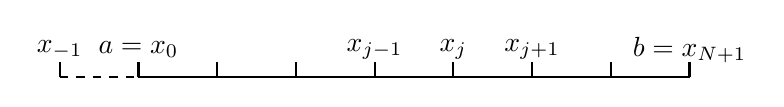
\begin{tikzpicture}
  \draw[color=black, thick](0,0) -- (1, 0) -- (2, 0) -- (3, 0) -- (4, 0) -- (5, 0) -- (6, 0) -- (7, 0);
  
   \draw[color=black, thick, dashed](-1, 0) -- (0,0);
  \foreach \x in {-1,...,7}
  {
  \draw[color=black, thick] (\x, 0) -- (\x, 0.2);
  }
  \node at (-1, 0.35) {$x_{-1}$};
  \node at (0, 0.35) {$a = x_0$};
    \node at (7, 0.35) {$b = x_{N+1}$};
     \node at (3, 0.35) {$ x_{j-1}$};
      \node at (4, 0.35) {$ x_{j}$};
       \node at (5, 0.35) {$x_{j+1}$};

\end{tikzpicture}

\end{center}



Apply ODE at $x_0$ and use central difference on BC to eliminate $u_{-1}$:
\begin{equation*}
	\begin{array}{r}
		 \frac{u_{-1}-2u_0+u_1}{h^2}+{p}_0\left(\frac{u_1-u_{-1}}{2h}\right) + q_0 u_0 = r_0\\
		 \frac{u_1-u_{-1}}{2h}=\alpha 
	\end{array}
\end{equation*}

\[\Rightarrow \frac{-2u_0+2u_1}{h^2} + q_0 u_0 = r_0 - {p}_0\alpha + \frac{2\alpha}{h} \]



%
%\begin{equation*}
%        \left. \begin{array}{rr}
%           \frac{u_{-1}-2u_0+u_1}{h^2}+{p}_0\left(\frac{u_1-u_{-1}}{2h}\right) + q_0 u_0 = r_0\\
%            u'(x_0)=\alpha  \frac{u_1-u_{-1}}{2h}=\alpha, 
%\ u_{-1} = u_1 -2\alpha h &\text{otherwise}
%        \end{array} \right\}
%        
%       % \frac{-2u_0+2u_1}{h^2} + q_0 u_0 = r_0 - {p}_0\alpha + \frac{2\alpha}{h}.
%
%    \end{equation*}

\end{frame}



%-=-=-=-=-=-=-=-=-=-=-=-=-=-=-=-=-=-=-=-=-=-=-=-=
%	FRAME:
%-=-=-=-=-=-=-=-=-=-=-=-=-=-=-=-=-=-=-=-=-=-=-=-=


\appendix



\end{document}
